\appendix
\addcontentsline{toc}{part}{Annexe}
%\markboth{\textbf{Annexe}}{}
\thispagestyle{empty}
\chapter{Les modèles IRT en code Stan.}


\begin{lstlisting}[language=Stan,caption={Code Stan pour le modèle de Rasch},basicstyle=\scriptsize, frame=lines,framesep=4.5mm,framexleftmargin=2.5mm,tabsize=2,numbers=left,fillcolor=\color{white},rulecolor=\color{black},numberstyle=\normalfont\scriptsize\color{black}]
    _1pl_model = """
    data {
        // numbers of things
        int<lower=1> N;  // number of observations
        int<lower=1> I;  // items,  number of questions  
        int<lower=1> S;  // subjects,  number of users 
        // data
        int<lower=1,upper=I> item[N];
        int<lower=1,upper=S> subject[N];
        int<lower=0,upper=1> grade[N];
        // data for posterior prediction using new data also used for Cross-validation
        int<lower=1> N_new;
        int<lower=1,upper=I> item_new[N_new];
        int<lower=1,upper=S> subject_new[N_new];
    }
    parameters {
        // parameters
        real ability[S];             //  alpha: ability of student
        real difficulty[I];          //  beta: difficulty of question
        real delta;                   // mean student ability
    }
    model {
        ability ~ normal(0,1);         
        difficulty ~ normal(0,1);   
        delta ~ normal(0.75,1);
        for(n in 1:N)
            grade[n] ~ bernoulli_logit(ability[subject[n]] - difficulty[item[n]] + delta);
    }
    generated quantities {
        int<lower=0,upper=1> y_pred[N];
        int<lower=0,upper=1> yNew_pred[N_new];
        vector[N] log_lik;

        for(n in 1:N){
            y_pred[n] = bernoulli_logit_rng(ability[subject[n]] - difficulty[item[n]] + delta);
            log_lik[n] = bernoulli_logit_lpmf( grade[n] | ability[subject[n]] - difficulty[item[n]]
            + delta);
        }
        for (n in 1:N_new) {
            yNew_pred[n] = bernoulli_logit_rng(ability[subject_new[n]] - difficulty[item_new[n]] + delta);                                             
        }
    }
    """
\end{lstlisting}
\newpage

\begin{lstlisting}[language=Stan,caption={Code Stan pour 2PL},basicstyle=\scriptsize, frame=lines,framesep=4.5mm,framexleftmargin=2.5mm,tabsize=2,numbers=left,fillcolor=\color{white},rulecolor=\color{black},numberstyle=\normalfont\scriptsize\color{black}]
    _2pl_model = """
    data {
        // numbers of things
        int<lower=1> N;  // number of observations
        int<lower=1> I;  // items,  number of questions  
        int<lower=1> S;  // subjects,  number of users 
        // data
        int<lower=1,upper=I> item[N];
        int<lower=1,upper=S> subject[N];
        int<lower=0,upper=1> grade[N];
        // data for posterior prediction using new data also used for Cross-validation
        int<lower=1> N_new;
        int<lower=1,upper=I> item_new[N_new];
        int<lower=1,upper=S> subject_new[N_new];
    }
    parameters {
        // parameters
        real ability[S];             //  alpha: ability of student
        real difficulty[I];          //  beta: difficulty of question
        vector<lower=0>[I] discrimination;      // discrimination of question
        real delta;                   // mean student ability
    }
    model {
        ability ~ normal(0,1);         
        difficulty ~ normal(0,1);   
        discrimination ~ lognormal(0,1);
        delta ~ normal(0.75,1);
        grade ~ bernoulli_logit(discrimination[item] .* (ability[subject] - (difficulty[item] + delta)));	
    }
    generated quantities {
        int<lower=0,upper=1> y_pred[N];
        int<lower=0,upper=1> yNew_pred[N_new];
        vector[N] log_lik;

        for(n in 1:N){
            y_pred[n] = bernoulli_logit_rng(discrimination[item[n]] * (ability[subject[n]] - (difficulty[item[n]] + delta)));
            log_lik[n] = bernoulli_logit_lpmf( grade[n] | discrimination[item[n]] * (ability[subject[n]] - (difficulty[item[n]] + delta)));
        }
        for (n in 1:N_new) {
            yNew_pred[n] = bernoulli_logit_rng(discrimination[item[n]] * (ability[subject_new[n]] - (difficulty[item_new[n]] + delta)));                             
        }
    }
    """
\end{lstlisting}

\newpage

\begin{lstlisting}[language=Stan,caption={Code Stan pour 3PL},basicstyle=\scriptsize, frame=lines,framesep=4.5mm,framexleftmargin=2.5mm,tabsize=2,numbers=left,fillcolor=\color{white},rulecolor=\color{black},numberstyle=\normalfont\scriptsize\color{black}]
    _3pl_model = """
    data {
        // numbers of things
        int<lower=1> N;  // number of observations
        int<lower=1> I;  // items,  number of questions  
        int<lower=1> S;  // subjects,  number of users 
        // data
        int<lower=1,upper=I> item[N];
        int<lower=1,upper=S> subject[N];
        int<lower=0,upper=1> grade[N];
        // data for posterior prediction using new data also used for Cross-validation
        int<lower=1> N_new;
        int<lower=1,upper=I> item_new[N_new];
        int<lower=1,upper=S> subject_new[N_new];
    }
    parameters {
        // parameters
        real ability[S];             //  alpha: ability of student
        real difficulty[I];          //  beta: difficulty of question
        vector<lower=0>[I] discrimination;      // discrimination of question
        vector<lower=0,upper=1>[I] guessing;    
        real delta;                   // mean student ability
    }
    model {
        ability ~ normal(0,1);         
        difficulty ~ normal(0,1);   
        discrimination ~ lognormal(0,1);
        guessing ~ beta(5,17);
        delta ~ normal(0.75,1);
        grade ~ bernoulli(guessing[item] + ((1-guessing[item]).*(inv_logit(discrimination[item] .* (ability[subject] - (difficulty[item] + delta))))));
    }
    generated quantities {
        int<lower=0,upper=1> y_pred[N];
        int<lower=0,upper=1> yNew_pred[N_new];
        vector[N] log_lik;

        for(n in 1:N){
            y_pred[n] = bernoulli_rng(guessing[item[n]] + ((1-guessing[item[n]]) * (inv_logit(discrimination[item[n]] .* (ability[subject[n]] - (difficulty[item[n]] + delta))))));
            log_lik[n] = bernoulli_lpmf( grade[n] | guessing[item[n]] + ((1-guessing[item[n]]) * (inv_logit(discrimination[item[n]] .* (ability[subject[n]] - (difficulty[item[n]] + delta))))));
        }
        for (n in 1:N_new) {
            yNew_pred[n] = bernoulli_rng(guessing[item[n]] + ((1-guessing[item[n]]) * (inv_logit(discrimination[item[n]] .* (ability[subject[n]] - (difficulty[item[n]] + delta))))));                                             
        }
    }
    """
\end{lstlisting}

\begin{lstlisting}[language=Stan,caption={Code Stan pour le modèle de Rasch avec cross-validation},basicstyle=\scriptsize, frame=lines,framesep=4.5mm,framexleftmargin=2.5mm,tabsize=2,numbers=left,fillcolor=\color{white},rulecolor=\color{black},numberstyle=\normalfont\scriptsize\color{black}]
    _1pl_cross_val_model = """
    functions {
        int[] permutation_rng(int N) {
            int y[N];
            for (n in 1:N)
                y[n] = n;
            vector[N] theta = rep_vector(1.0 / N, N);
            for (n in 1:N){
                int i = categorical_rng(theta);
                int temp = y[n];
                y[n] = y[i];
                y[i] = temp;
            }
            return y;
        }
    }
    
    data {
      // numbers of things
      
      int<lower=1> N;  // number of observations
      int<lower = 0, upper = N> N_test;
      int<lower=1> I;  // items,  number of questions  
      int<lower=1> S;  // subjects,  number of users
      
      // data
      
      int<lower=1,upper=I> item[N];
      int<lower=1,upper=S> subject[N];
      int<lower=0,upper=1> grade[N];
    }
    transformed data {
      int N_train = N - N_test;
      int permutation[N] = permutation_rng(N);
      // train
      int item_train[N_train] = item[permutation[1 : N_train]];
      int subject_train[N_train]  = subject[permutation[1 : N_train]];
      int grade_train[N_train]  = grade[permutation[1 : N_train]];
      int s_train = size(subject_train);
      int i_train = size(item_train);
      
      
      // test
      int item_test[N_test] = item[permutation[N_train + 1 : N]];
      int subject_test[N_test] = subject[permutation[N_train + 1 : N]];
      int grade_test[N_test] = grade[permutation[N_train + 1 : N]];
    }
    parameters {
      // parameters
      real ability[s_train];             //  alpha: ability od student
      real difficulty[i_train];          //  beta: difficulty of question
      real delta;                   // man student ability
      
    }
    model {
    
      ability ~ normal(0,1);         
      difficulty ~ normal(0,1);   
      delta ~ normal(0.75,1);
      
      for (n in 1:N_train) {
          grade_train[n] ~ bernoulli_logit(ability[subject_train[n]] - difficulty[item_train[n]] + delta);
      }
      
    }
    generated quantities {
      int<lower=0,upper=1> grade_pred[N_test];
      int<lower=0,upper=1> grade_observed[N_test];
      grade_observed = grade_test;
      
      for (n in 1:N_test) {
        grade_pred[n] = bernoulli_logit_rng(ability[subject_test[n]] - difficulty[item_test[n]] + delta);
      }
    }
    """
\end{lstlisting}

\chapter{Les distributions des modèles.}

\begin{figure}[H]
	\begin{center}
		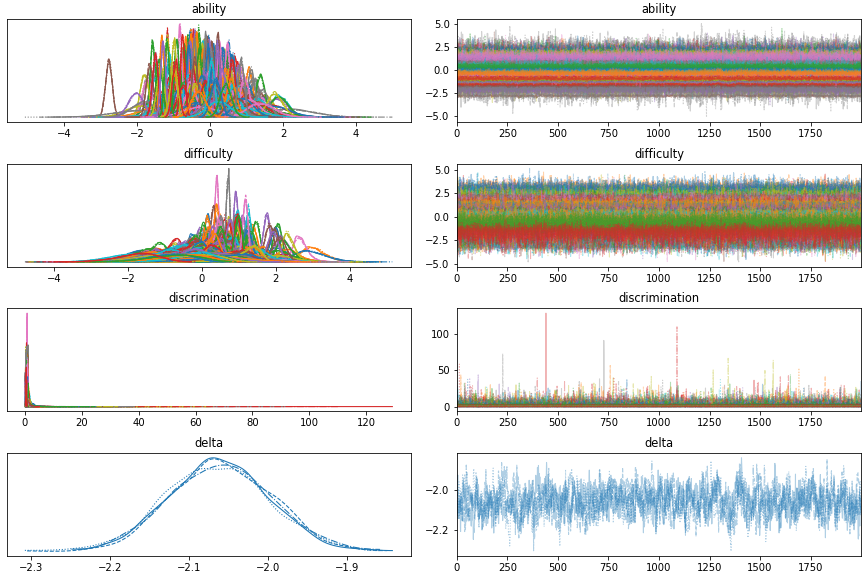
\includegraphics[width=\textwidth]{images/annexe/model_plot-trace2.png}
	\end{center}
	\caption{Les distributions postérieures du modèle logistique à deux paramètres.}
	\label{model_trace-plot2}
\end{figure}

\begin{figure}[H]
	\begin{center}
		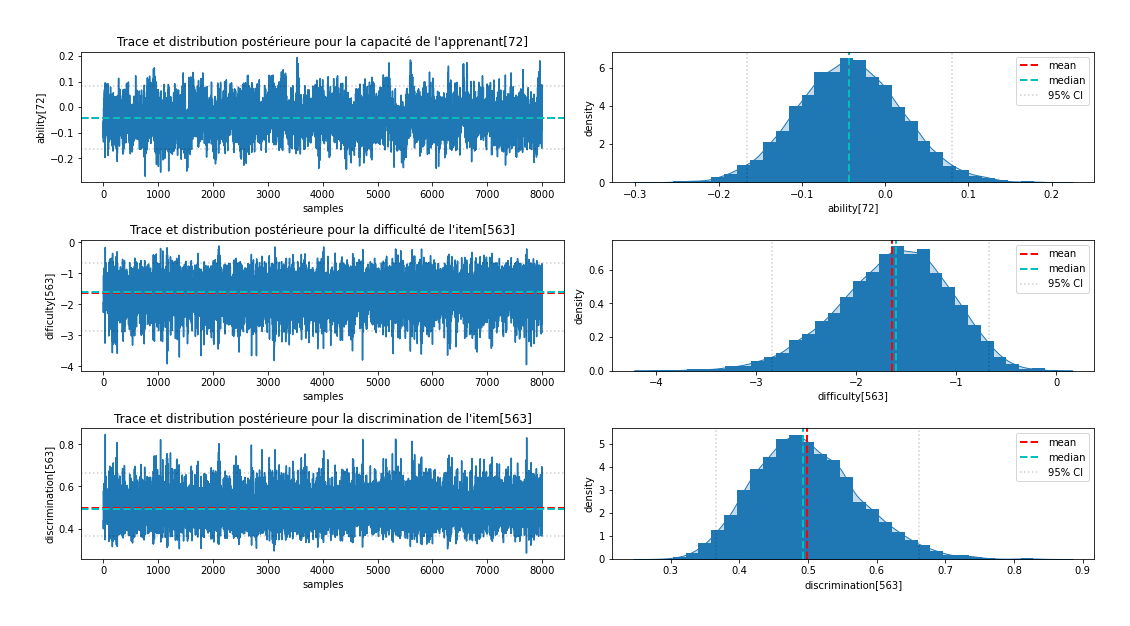
\includegraphics[width=\textwidth]{images/annexe/params_posterior_distribution2.png}
	\end{center}
	\caption{Distribution postérieure de la capacité de l’apprenant[72], de la difficulté de l’item[563] et de la discrimination de l’item[563] du modèle 2PL.}
	\label{params_posterior_distribution_2pl}
\end{figure}

\begin{figure}[H]
	\begin{center}
		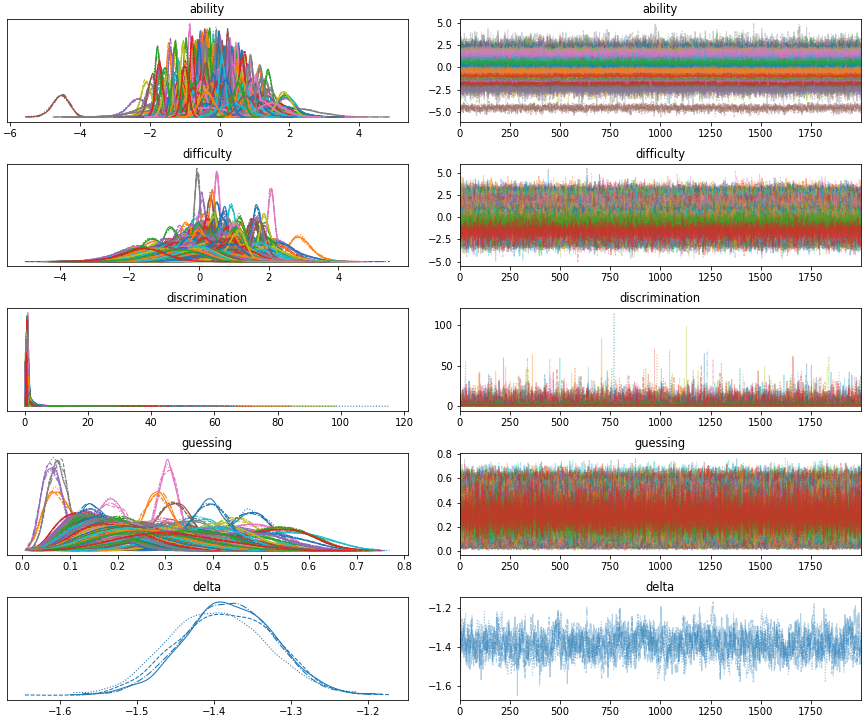
\includegraphics[width=\textwidth]{images/annexe/model_plot-trace3.png}
	\end{center}
	\caption{Les distributions postérieures du modèle logistique à trois paramètres.}
	\label{model_trace-plot3}
\end{figure}

\begin{figure}[H]
	\begin{center}
		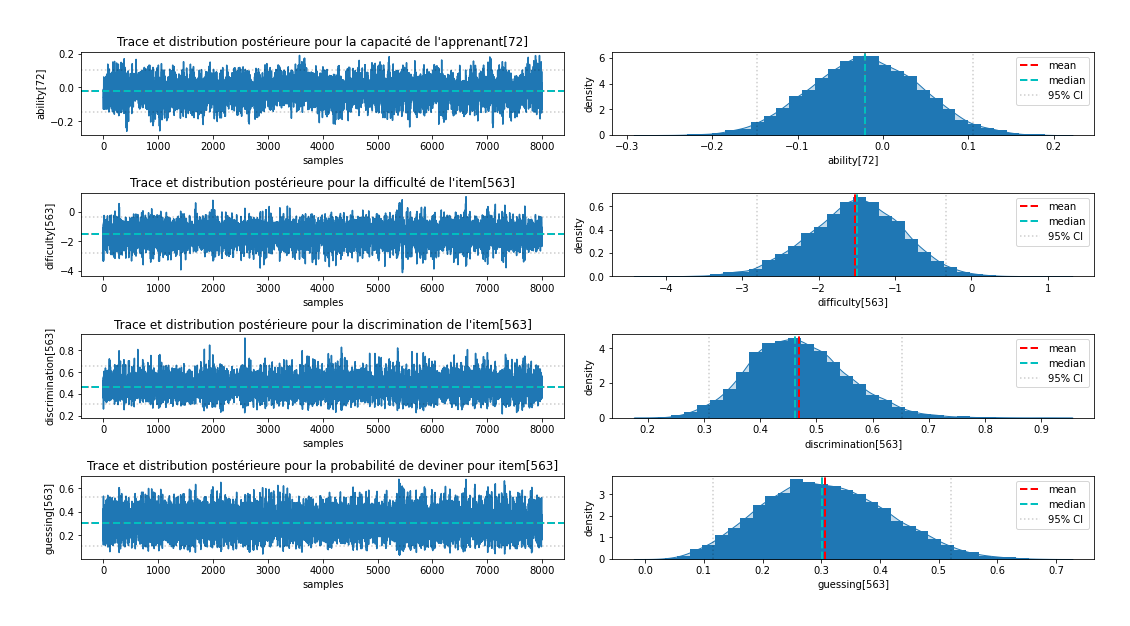
\includegraphics[width=\textwidth]{images/annexe/params_posterior_distribution3.png}
	\end{center}
	\caption{Distribution postérieure de la capacité de l’apprenant[72], de la difficulté de l’item[563], de la discrimination de l’item[563] et de la chance de deviner la reponse correcte de l'item[563] du modèle 2PL.}
	\label{params_posterior_distribution_3pl}
\end{figure}

\chapter{Comparaison des résultats utilisant les scores observés et les scores prédit par les modèles IRT.}

\begin{figure}[H]
    \centering
    \subfloat[\centering Visualisation en 2D des deux premières composantes de la matrice de similarité créer avec les scores observés.]{{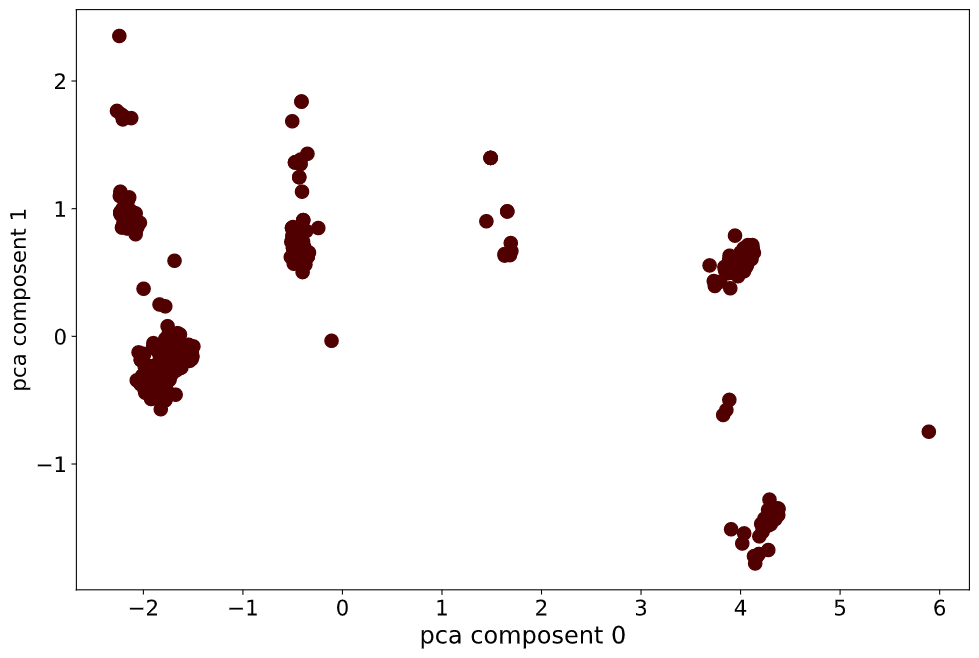
\includegraphics[width=7cm]{images/chapitre7/features_plot.png}}}%
    \qquad
    \subfloat[\centering Visualisation en 2D des deux premières composantes de la matrice de similarité créer avec les scores prédit par les modèles IRT.]{{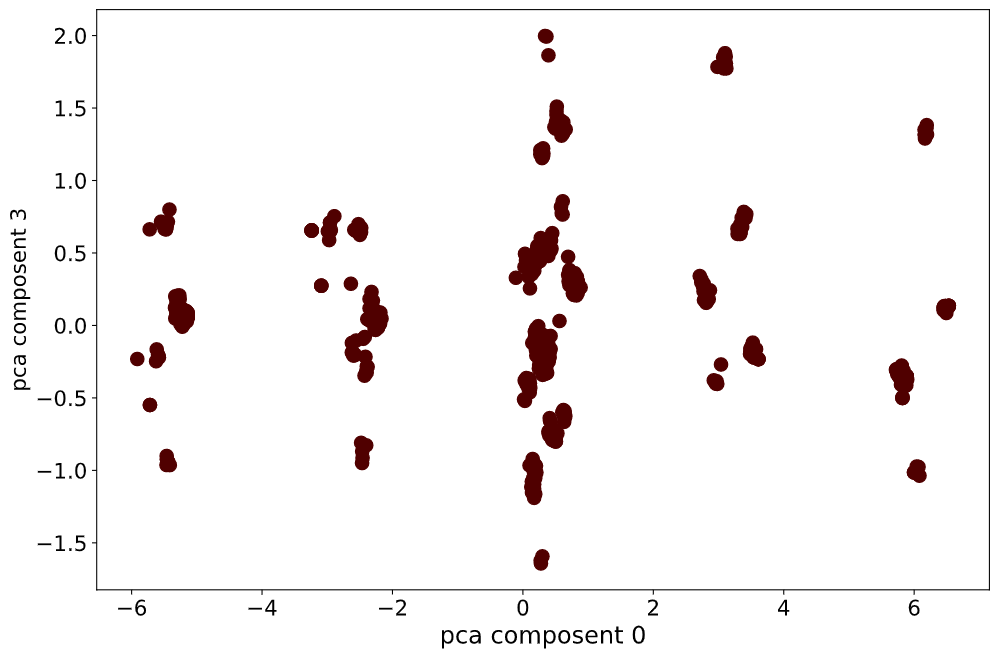
\includegraphics[width=7cm]{images/chapitre7/features_plot1.png} }}%
    %\caption{Dendrogramme}%
\end{figure}

\begin{figure}[H]
    \centering
    \subfloat[\centering Le dendrogramme utilisant la méthode de liaison « average » de la matrice de similarité créer avec les scores observés.]{{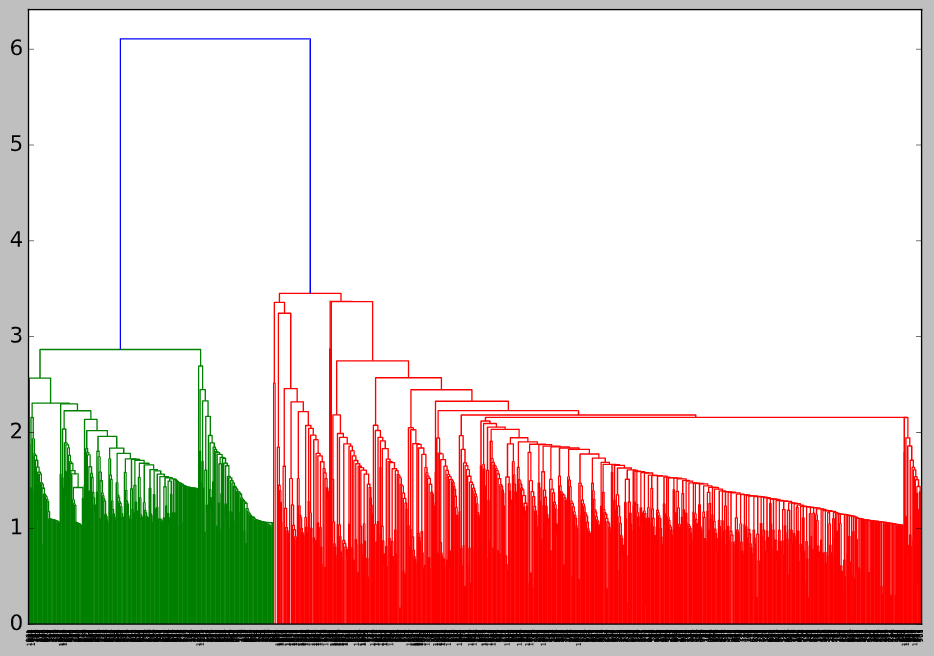
\includegraphics[width=7cm]{images/chapitre7/dendrogram_of_dataset.png}  }}%
    \qquad
    \subfloat[\centering Le dendrogramme utilisant la méthode de liaison « average » de la matrice de similarité créer avec les prédit par les modèles IRT.]{{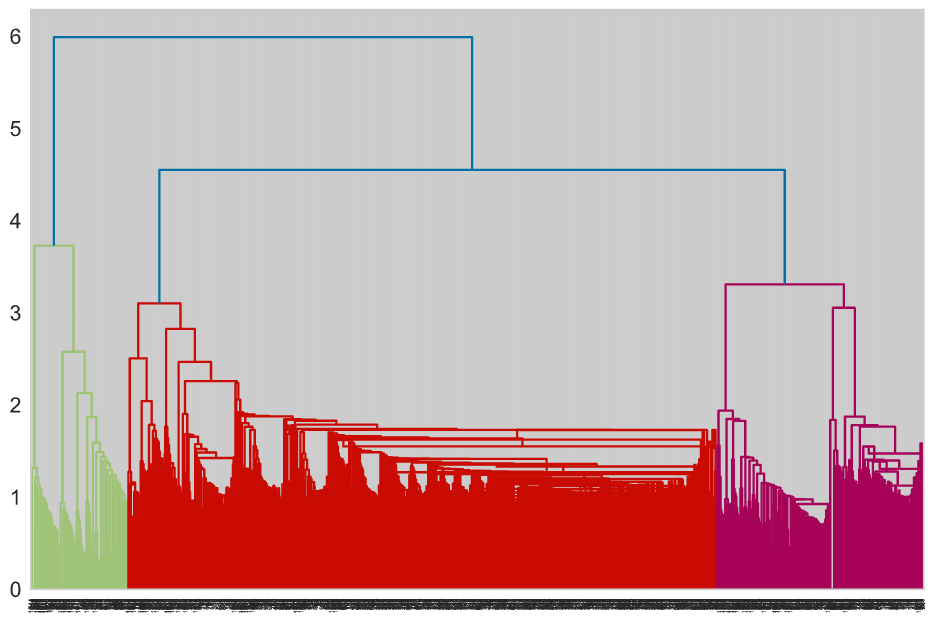
\includegraphics[width=7cm]{images/chapitre7/dendrogram_of_dataset1.png} } }%
    %\caption{Dendrogramme}%
\end{figure}

\newpage

\begin{figure}[H]
	\begin{center}
		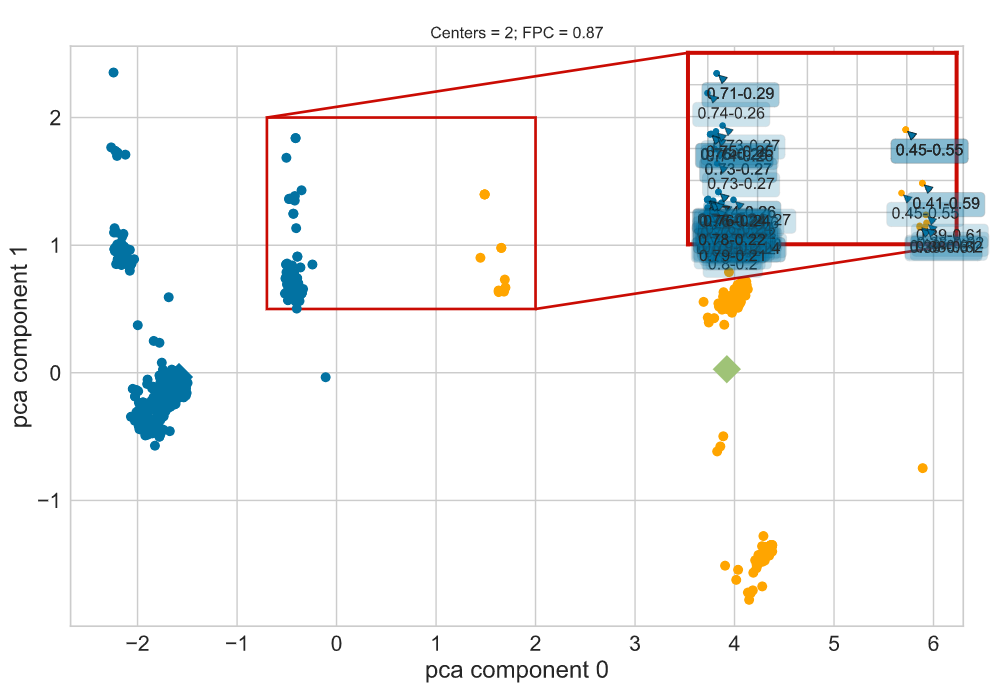
\includegraphics[width=\textwidth]{images/chapitre7/fuzzy_partition_plot.png}
	\end{center}
	\caption{Visualisation des clusters de la méthode fuzzy et le degré d’appartenance des items à chaque cluster utilisant la matrice de similarité créer avec les prédit par les modèles IRT.}
	\label{fuzzy_partition_plot0}
\end{figure}

\newpage

\vspace{2em}
\begin{table}[H]
	\centering
	\addtolength{\leftskip} {-4cm}
	\addtolength{\rightskip}{-4.5cm}
	\begin{tabular}{|m{2cm}|m{2cm}|m{2cm}|m{2cm}|m{2cm}|m{3cm}|}
	\hline
	\rowcolor{blueforest}
	\multicolumn{6}{|m{16cm}|}{\centering \color{white} \textbf{Kmeans clustering} } \\ \hline
	&  \multicolumn{4}{|m{8cm}|}{\centering \textbf{Indice de validité} } & \\ \hline
	\textbf{Nombre de clusters}  &   \textbf{Indice de Dunn} & \textbf{Indice Calinski Harabasz}& \textbf{Indice Davies-Bouldin} & \textbf{Silhouette score}  &  \textbf{Nombre d'items dans un cluster }\\ \hline
	2  & 0.43  & \cellcolor{gray!40} 2414  & \cellcolor{gray!40} 0.58   &  \cellcolor{gray!40} 0.62   & 308  \(\displaystyle \thicksim  \) 776  \\ \hline %\cellcolor{gray!40}
	3  & \cellcolor{gray!40} 0.51  & 1452  & 1.05   &  0.44   & 68   \(\displaystyle \thicksim  \) 719  \\ \hline
	4  & 0.50  & 1126  & 1.21   &  0.38   & 68   \(\displaystyle \thicksim  \) 719  \\ \hline
	5  & 0.47  & 937   & 1.27   &  0.306  & 52   \(\displaystyle \thicksim  \) 667  \\ \hline
	6  & 0.46  & 810   & 1.30   &  0.295  & 43   \(\displaystyle \thicksim  \) 624  \\ \hline
	7  & 0.45  & 711   & 1.33   &  0.285  & 33   \(\displaystyle \thicksim  \) 591  \\ \hline
	8  & 0.45  & 626   & 1.29   &  0.289  & 7    \(\displaystyle \thicksim  \) 591  \\ \hline
	9  & 0.38  & 566   & 1.33   &  0.26   & 7    \(\displaystyle \thicksim  \) 564  \\ \hline
	10 & 0.37  & 527   & 1.47   &  0.24   & 7    \(\displaystyle \thicksim  \) 564  \\ \hline \hline
	\rowcolor{blueforest}
	\multicolumn{6}{|m{16cm}|}{\centering \color{white} \textbf{Agglomérative clustering} } \\ \hline
	&  \multicolumn{4}{|m{8cm}|}{\centering \textbf{Indice de validité} } & \\ \hline
	\textbf{Nombre de clusters}  &   \textbf{Indice de Dunn} & \textbf{Indice Calinski Harabasz}& \textbf{Indice Davies-Bouldin} & \textbf{Silhouette score}  &  \textbf{Nombre d'items dans un cluster }\\ \hline
	2  & \cellcolor{gray!40} 0.57 & \cellcolor{gray!40} 2368 & \cellcolor{gray!40} 0.58   & \cellcolor{gray!40} 0.62    &  297  \(\displaystyle \thicksim  \)  787  \\ \hline 	
	3  & 0.51 & 1452 & 1.05   & 0.44    &  68   \(\displaystyle \thicksim  \)  719  \\ \hline
	4  & 0.48 & 974  & 1.054  & 0.43    &  2    \(\displaystyle \thicksim  \)  717  \\ \hline
	5  & 0.48 & 733  & 0.937  & 0.41    &  1    \(\displaystyle \thicksim  \)  716  \\ \hline
	6  & 0.48 & 594  & 0.933  & 0.38    &  1    \(\displaystyle \thicksim  \)  716  \\ \hline
	7  & 0.48 & 506  & 0.9366 & 0.354   &  1    \(\displaystyle \thicksim  \)  716  \\ \hline
	8  & 0.48 & 435  & 0.80   & 0.352   &  1    \(\displaystyle \thicksim  \)  716  \\ \hline
	9  & 0.56 & 444  & 0.89   & 0.34    &  1    \(\displaystyle \thicksim  \)  716  \\ \hline
	10 & 0.52 & 438  & 0.95   & 0.30    &  1    \(\displaystyle \thicksim  \)  666  \\ \hline \hline
	\rowcolor{blueforest}
	\multicolumn{6}{|m{16cm}|}{\centering \color{white} \textbf{Fuzzy clustering} } \\ \hline
	&  \multicolumn{4}{|m{8cm}|}{\centering \textbf{Indice de validité} } & \\ \hline
	\textbf{Nombre de clusters}  &   \textbf{FPC} & \textbf{Indice Calinski Harabasz}& \textbf{Indice Davies-Bouldin} & \textbf{Silhouette score}  &  \textbf{Nombre d'items dans un cluster }\\ \hline
	2  & \cellcolor{gray!40} 0.865 & \cellcolor{gray!40} 2413.6  & \cellcolor{gray!40} 0.59   &  \cellcolor{gray!40} 0.62    &  308 \(\displaystyle \thicksim  \)  776  \\ \hline 	
	3  & 0.54  & 1378    & 1.27   &  0.40    &  71  \(\displaystyle \thicksim  \)  705 \\ \hline
	4  & 0.45  & 1394    & 1.02   &  0.53    &  1   \(\displaystyle \thicksim  \)  776 \\ \hline
	5  & 0.35  & 708.51  & 2.30   &  -0.008  &  3   \(\displaystyle \thicksim  \)  757 \\ \hline
	6  & 0.30  & 697     & 3.06   &  0.024   &  1   \(\displaystyle \thicksim  \)  766 \\ \hline
	7  & 0.26  & 486.75  & 4.2    &  0.011   &  6   \(\displaystyle \thicksim  \)  735 \\ \hline
	8  & 0.23  & 481.55  & 4.29   &  -0.022  &  1   \(\displaystyle \thicksim  \)  685 \\ \hline
	9  & 0.20  & 666     & 2.57   &  0.21    &  1   \(\displaystyle \thicksim  \)  680 \\ \hline
	10 & 0.18  & 408     & 3.72   &  -0.0094 &  1   \(\displaystyle \thicksim  \)  726 \\ \hline
  \end{tabular}
	\caption{Résultats des indices de validité du clustering utilisant la matrice de similarité créer avec les prédit par les modèles IRT.}
	\label{clusters_indice_score0}
\end{table}
